\subsection{Etude de $\int_x^{x^2} \frac{dt}{\ln(t)}.$ (Pb) }

\begin{exercice}
Le but de ce problème est d'étudier la fonction définie par : 
$$g : x \mapsto \int_x^{x^2} \frac{dt}{\ln(t)}.$$
\begin{enumerate}
\item Etude globale : 
\begin{enumerate}
\item Justifier que $g$ est bien définie sur $\cD_g = ]0,1[\cup ]1,+\infty[$. 
\item Montrer que $g$ est positive sur $\cD_g$. 
\item Justifier que $g$ est dérivable sur $\cD_g$  et exprimer sa dérivée en tout point de $\cD_g$. 
\item Montrer que $g$ est de classe $\cC^\infty$ sur $\cD_g$. 
\item Etudier les variations de $g$ sur $\cD_g$. (les limites aux bornes ne sont pas demandées pour cette question) 
\end{enumerate}
\item Etude au voisinage de $0$
\begin{enumerate}
\item Montrer que :
$$\forall x\in ]0,1[\quad \frac{x(x-1)}{2\ln(x)}\leq g(x)\leq \frac{x(x-1)}{\ln(x)}$$
On fera très attention aux signes dans les inégalités. 
\item En déduire que $g$ se prolonge par continuité en $0$ et préciser la valeur de ce prolongement. 
Par la suite, on note encore $g$ la fonction continue, prolongée en $0$
\item Montrer que $g$ est dérivable à droite en $0$ et préciser $g'(0)$. 
\end{enumerate}
\item Etude au voisinage de $1$.
\begin{enumerate}
\item A l'aide du théorème des accroissements finis appliquer à $h(t) =\ln(t) -t$ montrer que pour tout $t\in ]0,1[ $ :
$$0\leq \frac{\ln(t) - t+ 1 }{t-1}\leq \frac{1-t}{t} $$
\item En déduire que pour tout $t\in ]0,1[ $ :
$$\left|\frac{\ln(t) - t+ 1 }{t-1}\right|\leq \left|\frac{1-t}{t}\right|.$$
\item Montrer de manière analogue que pour tout $t>1$ on  a
$$\left|\frac{\ln(t) - t+ 1 }{t-1}\right|\leq \left|\frac{1-t}{t}\right|.$$

\item En déduire qu'il existe $\eta >0 $ tel que pour tout $t  \in [1-\eta, 1+\eta]$ 
$$\left|\frac{1}{\ln(t)} -\frac{1}{t-1}\right|\leq 2$$
\item Conclure  que $g$  est prolongeable par continuité en $1$. 
\end{enumerate}

\item Etude au voisinage de $+\infty$.
\begin{enumerate}
\item Montrer que :
$$\forall x\in ]1,+\infty[\quad \frac{x(x-1)}{2\ln(x)}\leq g(x)$$
\item En déduire la limite de $g$ en $+\infty$. 
\end{enumerate}
\end{enumerate}
\end{exercice}

\begin{correction}
\begin{enumerate}
\item Etude globale
\begin{enumerate}
\item On note $f$ la fonction définie par $f(x)=\frac{1}{\ln(x)}$.
Cette fonction est définie pour tout $x\in \R$ tel que $\ln(x)$ soit défini, c'est-à-dire $x>0$ et tel que $\ln(x)\neq0$, c'est-à-dire $x\neq 1$. On a donc $D_f =  ]0,1[\cup ]1,+\infty[$. 
La fonction $f$ est continue  sur son ensemble de définition comme quotient de fonction usuelle, elle admet donc une primitive sur $]0,1[$ et sur $]1,+\infty[$. \footnote{Il faut faire attention ici que \underline{l'intervalle} définie par les bornes de l'intégrale ne contiennent pas des points où $f$ n'est pas définie. } Notons $F_1$ une primitive sur $]0,1[$. Pour tout $x\in ]0,1[$, on a $x^2\in ]0,1[$ et ainsi $g(x)=F_1(x^2)-F_1(x)$ est bien définie sur $]0,1[$. 
De la même façon, en notant $F_2$ une primitive sur $]1,+\infty[$. Pour tout $x\in ]1,\infty[$, on a $x^2\in ]1,\infty[$ et ainsi $g(x)=F_2(x^2)-F_2(x)$ est bien définie sur $]1,\infty[$. 

\item 
Nous reprenons les notations de la question 1. Pour tout $x\in ]0,1[, $ $x^2<x$ ainsi $g(x) = -\int_{x^2}^x f(t)dt$, où les bornes d'intégration sont ordonnées dans le sens croissant. Maintenant pour $x\in ]0,1[$,  $[x^2,x] \subset ]0,1[$ or pour $t\in ]0,1[$, $f(t) < 0$. Ainsi $g(x)>0$ sur $]0,1[$. 

Pour $x>1$, on a $x^2>x$ et les bornes sont déjà bien ordonées. De plus $\frac{1}{\ln(t)}>0$ pour tout $t>1$ et on a bien $g(x)>0$ sur $]1,+\infty[$. 

\item Nous reprenons les notations de la question 1. Par définition on  a
$g(x) = F_1 (x^2) - F_1(x)$ pour $0<x<1$ et $g(x) = F_2 (x^2) - F_2(x)$ pour $x>1$. Or par définition d'une primitive les fonctions $F_1, F_2$ sont dérivables sur leur ensemble de définition. Donc $g$ est dérivable en tant que composée et somme de fonctions dérivables. 

On  a pour tout $x<1$ : $g'(x) = 2xF_1'(x^2) - F_1'(x)$. Or $F_1'(x) =f(x)$ et donc 
$g'(x) =\frac{2x}{\ln(x^2)}-\frac{1}{\ln(x)},  $ en simplifiant et factorisant on obtient : 
$$g'(x) = \frac{x-1}{\ln(x)}$$

Les calculs sont identiques sur $]1,+\infty[$. 

\item La fonction $g'$ est de classe $\cC^\infty$ sur $\cD_g$ comme quotient de fonction $\cC^\infty$. Ainisi $g$ est de classe $\cC^\infty$ sur $\cD_g$. 

\item On  a vu que pour tout $x\in \cD_g$ on a 
$$g'(x) = \frac{x-1}{\ln(x)}$$
On obtient le tableau de signe/variations suivant :

\begin{tikzpicture}
   \tkzTabInit{$x$ / 1 , $x-1$ / 1, $\ln(x)$ / 1, $g'(x)$/1, $g(x)$ /1.5 }{$0$, $1$, $+\infty$}
   \tkzTabLine{, -, z, +, }
      \tkzTabLine{, -, z, +, }
            \tkzTabLine{, +, d, +, }
           
\tkzTabVar{-/ , R/, +/ }
 \tkzTabIma{1}{3}{2}{  }
  % \tkzTabVal{1}{2}{0.5}{}{} 
\end{tikzpicture}





\end{enumerate}
\item Etude au voisinage de $0$. 
\begin{enumerate}
\item Soit $x\in ]0,1[$, alors comme on l'a vu précédemment 
$g(x)  = -\int_{x^2}^x f(t)dt$ où les bornes de l'intégrales sont bien ordonnées. 
Par ailleurs pour tout $t\in [x^2,x]$ on a $\ln(x^2)\leq \ln(t) \leq \ln(x)<0$ par croissance du logarithme. Et donc 
$$\frac{1}{\ln(x)}\leq \frac{1}{\ln(t)}\leq \frac{1}{\ln(x^2)}$$ par décroissance de la fonction $x\tv \frac{1}{x}$ sur $R^*_-$

Par croissance de l'intégrale on obtient alors : 

$$\int_{x^2}^x \frac{1}{\ln(x)}dt \leq \int_{x^2}^x \frac{1}{\ln(t)}dt\leq \int_{x^2}^x \frac{1}{\ln(x^2)}dt$$
Remarquons que le membre le plus à gauche et le plus à droite sont des fonctions constantes vis-à-vis de $t$. Ainsi leur intégrale ce calcule immédiatement, on obtient  

$$(x-x^2) \frac{1}{\ln(x)} \leq  \int_{x^2}^x \frac{1}{\ln(t)}dt\leq (x-x^2)\frac{1}{\ln(x^2)}$$
Le terme du milieu correspond à $-g(x)$ et on a donc  après multiplication par $-1$
qui inverse le sens des inégalités ont obtient : 
$$ (x^2-x) \frac{1}{\ln(x^2)}\leq g(x)\leq (x^2-x) \frac{1}{\ln(x)}$$
c'est-à-dire en factorisant : 
$$ \frac{x(x-1)}{2\ln(x)}\leq g(x)\leq \frac{x(x-1)}{\ln(x)}$$


\item Par calcul usuel sur les limites : $\lim_{x\tv 0} \frac{x)}{\ln(x)} =0$ ainsi 
$$\lim_{x\tv 0}  \frac{x(x-1)}{2\ln(x)} =\lim_{x\tv 0}  \frac{x(x-1)}{\ln(x)} =0$$
Le théorème des gendarmes assure que $g$ admet une limite en $0$ et 
$$\lim_{x\tv 0} g(x) =0$$
$g$ est donc prolongeable par continuité en posant $g(0)=0$

\item On calcule le taux d'accroissement en $0$ : 
$\tau_{g,x}   =\frac{g(x)-g(0)}{x-0}= \frac{g(x)}{x}$
Ainsi pour tout $x\in ]0,1[$: 
$$ \frac{x-1}{2\ln(x)}\leq \tau_{g,x}\leq \frac{x-1}{\ln(x)}$$
Comme $\lim_{x\tv 0} \frac{1)}{\ln(x)} =0$, de nouveau d'après le théorème des gendarmes on a : $\lim_{x\tv 0} \tau_{g,x}  =0$ et ainsi $g$ est dérivable en $0$ et on a $g'(0) = 0$. 




\end{enumerate}
\item Au voisinage de $1$. 
\begin{enumerate}
\item 
On applique le théorème des accroissements finis à la fonction $h(x) = \ln(x) -x$ sur l'intervalle $[t,1]$ (ou $[1,t]$ selon l'ordre de $1$ par rapport à $x$). 
$h $ est continue sur $\R_+^*$ donc en particulier sur $[t,1]$. $h$ est $\cC^1$ sur $\R_+^*$ donc en particulier sur $]t,1[$. Ainsi, il existe $c\in ]t,1[$  tel que 
$$\frac{h(t)-h(1)}{t-1}=h'(c) $$
Pour tout 
$h'(x) = \frac{1}{x}-1$, on a donc 
$$\frac{\ln(t)- t +1}{t-1} =\frac{1-c}{c}$$

Pour tout $t<1$ et tout $c\in ]t,1[$  on  a 
$t<c<1 $ donc $1-t> 1-c >0$ et $\frac{1}{t}>\frac{1}{c}>1$ d'où 
$$\frac{1-t}{t} > \frac{1-c}{c}>0$$
En particulier on a 
$$0\leq \frac{\ln(t) - t+ 1 }{t-1}\leq \frac{1-t}{t} $$

\item  Comme pour tout $t\in ]0,1[$, $-\frac{1-t}{t}<0$ on a donc 
$$-\frac{1-t}{t} \leq \frac{\ln(t) - t+ 1 }{t-1}\leq \frac{1-t}{t} $$
c'est-à-dire 
$$\left|\frac{\ln(t) - t+ 1 }{t-1}\right|\leq \left|\frac{1-t}{t}\right|.$$


\item Le début du raisonement est similaire et on obtient qu'il existe $c\in [1,t]$ tel que $$\frac{\ln(t)- t +1}{t-1} =\frac{1-c}{c}$$

Remarquons que $a:t\mapsto \frac{1-t}{t}$ est une fonction décroissante sur $]1,+\infty[$ donc pour tout $t>1$ et tout $c\in ]1,t[$ on a 
$$a(t)\leq a(c) \leq a(c)$$
ainsi : 
$$\frac{1-t}{t}\leq \frac{1-c}{c}\leq 0 \leq-\frac{1-t}{t} $$
où la dernière inégalité provient du signe de $\frac{1-t}{t}$ sur $]1,+\infty[$. 
On a donc  :




$$\left|\frac{\ln(t) - t+ 1 }{t-1}\right|\leq -\frac{1-t}{t} =\left|\frac{1-t}{t}\right|.$$

\item 

$$\frac{1}{\ln(t)} -\frac{1}{t-1} = \frac{t-1 -\ln(t)}{\ln(t)(t-1)}$$
donc 


$$\left| \frac{1}{\ln(t)} -\frac{1}{t-1}\right| =\frac{1}{|\ln(t)|}\left|\frac{t-1 -\ln(t)}{(t-1)}\right|$$
et donc 
$$\left| \frac{1}{\ln(t)} -\frac{1}{t-1}\right| \leq \frac{1}{|\ln(t)|}\left|\frac{1-t}{t}\right|.$$

Or $\ddp \lim_{t\tv 1} \frac{|1-t|}{|\ln(t)|}=1$ grâce à l'équivalent $\ln(t+1) \sim_0 t$
Donc $\ddp \lim_{t\tv 1}  \frac{1}{|\ln(t)|}\left|\frac{1-t}{t}\right| = 1$ 
Ainsi d'après la définition de la limite en $1$, pour tout $\epsilon>0$, il existe $\eta>0 $ tel que pour tout $t\in [1-\eta, 1+\eta]$ on a 
$$ \left| \frac{1}{|\ln(t)|}\left|\frac{1-t}{t}\right|  -1 \right|\leq \epsilon$$
En particulier, en prenant $\epsilon=1$, il existe $\eta>0$ tel que  pour tout $t\in [1-\eta, 1+\eta]$ on a  
$ \left| \frac{1}{|\ln(t)|}\left|\frac{1-t}{t}\right|  -1 \right| \leq 1$
Ce qui donne notamment : 
$$\frac{1}{|\ln(t)|}\left|\frac{1-t}{t}\right|  -1  \leq 1$$ et enfin 
$$\frac{1}{|\ln(t)|}\left|\frac{1-t}{t}\right|  \leq   2$$

Avec l'inégalité obtenue précédemment on obtient bien qu'il existe $\eta>0$ tel que pour tout $t\in [1-\eta,1+\eta]$: 
$$\left| \frac{1}{\ln(t)} -\frac{1}{t-1}\right| \leq 2 $$

\item Regardons donc $u(x)= g(x) -\int_x^{x^2} \frac{1}{t-1} dt $ on obtient 
\begin{align*}
u(x) &= \int_x^{x^2} \frac{1}{\ln(t)} - \frac{1}{t-1} dt \quad \text{ par linéarité, d'où} \\
|u(x) |& = \left| \int_x^{x^2} \frac{1}{\ln(t)} - \frac{1}{t-1} dt\right| \\
|u(x)| &\leq \int_{[x, {x^2}]}  \left| \frac{1}{\ln(t)} - \frac{1}{t-1} \right|dt \quad{ En utilisant l'inégalité triangulaire}
\end{align*}
Remarquons ici que  $\int_{[x, {x^2}]}  $ signifie que l'on intégre sur $[x,x^2]$ ou $[x^2,x]$ selon l'ordre des bornes. On peut sinon faire une disjonction de cas, avec $x>1$ ou $x<1$. 

On a donc pour $x,x^2\in [1-\eta, 1+\eta]$ 
$$|u(x)| \leq \int_{[x, {x^2}]} 2dt = 2|x^2-x| $$  

Or quand $x\tv 1$, on a bien $x,x^2 \in   [1-\eta, 1+\eta]$  donc l'inégalité est vraie pour $x$ suffisament proche de $1$. 
Or $\lim_{x\tv 1} |x^2-x|=  0$ donc le théorème des gendarmes assure que 
$$\lim_{x\tv 1} |u(x) | =0$$

Or $\int_x^{x^2} \frac{1}{t-1}dt = [\ln(t)]_x^{x^2} = \ln(x^2) -\ln(x) =\ln(2)$
Ce qui donne avec la limite de $|u(x)|$, $\lim_{x\tv 1} |g(x)-\ln(2)| =0$ 
c'est-à-dire :
$$\lim_{x\tv 1} g(x) =\ln(2)$$
Ainsi $g$ est prolongeable par continuité en $1$ en posant $g(1)  = \ln(2)$ 

\end{enumerate}
\item Au voisinage de $+\infty$. 
\begin{enumerate}
\item On suit le même raisonnement que pour la question 2(a) : pour $x>1$ et pour $t\in [x,x^2]$ on a 
$$\frac{1}{\ln(x^2)} \leq \frac{1}{\ln(t)}\leq \frac{1}{\ln(x)}$$
par décroissance de la fonction $f$. 
Par positivité de l'intégrale on a donc :
$$\int_x^{x^2} \frac{1}{\ln(x^2)} dt \leq\int_x^{x^2}  \frac{1}{\ln(t)}dt$$
et ainsi 
$\frac{x^2-x}{\ln(x^2)}\leq g(x)$
d'où 
$$\frac{x(x-1)}{2\ln(x)}\leq g(x)$$

\item Par croissance comparée $\lim_{x\tv +\infty} \frac{x(x-1)}{2\ln(x)}= +\infty$ et donc d'après le théorème de comparaison on a : 
$$\lim_{x\tv +\infty}g(x) =+\infty$$


\end{enumerate}


\end{enumerate}
\end{correction}